\section{평가}\label{sec:eval}
0-LLM 결정론적 감사 계층과 제한된 확률적 제안기 파일럿을 분리 보고하며, 서로 다른 코호트와 분모는 통합하지 않는다.

\subsection{E1 오프라인 적합성 및 결정론적 경계 감사}
\textbf{E1}(게이트 픽스처 13건, 조건당 수리 12건)에서 네 조건 모두 구성 불변식(게이트 13/13, 무결성 결함 10/10)을 만족했다. 무효 수리 사례에서는 \texttt{rejection\_only}와 \texttt{unchanged\_retry}가 0/12, \texttt{WorldState}를 읽지 않는 유도 수리 $\rho$가 5/12, 상태 참조 오라클이 6/12를 복구했다.

단일 월드 픽스처를 넘어 권한 경계를 시험하기 위해, 방 개수(4, 8), 위상(잠긴 연쇄, 우회 분기), 열쇠 배치(4종), 퀘스트 단계(2종)를 교차한 32개 조합에 후보 13종을 적용해 조건당 416건(총 1,664건)과 표면 센티넬 48건(조건당 12건)을 평가했다.

\begin{table}[!tbp]
\caption{결정론적 권한 경계 감사 (조건당 416건 + 표면 센티넬 48건; 0 LLM 호출)}
\label{tab:boundary-full}
\centering
\footnotesize
\begin{tabularx}{\columnwidth}{@{}>{\raggedright\arraybackslash}X*{4}{>{\centering\arraybackslash}p{0.11\columnwidth}}@{}}
\toprule
\textbf{결과 (416/조건)} & \textbf{스키마} & \textbf{거부} & \textbf{재시도} & \textbf{유도 $\rho$} \\
\midrule
최초 무효 제안 & 260 & 260 & 260 & 260 \\
위험 최종 커밋 & 260 & \textbf{0} & \textbf{0} & \textbf{0} \\
수리 복구 (무효$\rightarrow$유효) & 0 & 0 & 0 & \textbf{128} \\
보류 (상태 불변) & 0 & 260 & 260 & 132 \\
목표 달성 & 124 & 124 & 124 & \textbf{252} \\
최초 유효 보존 (156건) & 156 & 156 & 156 & 156 \\
구조 서명 보존 (11종) & 11/11 & 11/11 & 11/11 & 11/11 \\
\bottomrule
\end{tabularx}
\end{table}

표~\ref{tab:boundary-full}에서 \texttt{schema\_only}는 무효 제안 260/416건을 커밋한 반면, 의미 게이트 조건은 오탐 0/156건과 폐쇄--BFS 32/32 일치 속에 0/416건만 커밋했다. 유도 수리 $\rho$는 128/260건을 복구해 목표 달성을 252/416건으로 높였다. 표면 센티넬에서는 명시적 금지 사실 6/6건을 차단했으나 미선언 우회 표현 6/6건은 통과했다.

\subsection{정보 공개 동등성, NPC 스크리닝 및 KG 시뮬레이션}
저작된 \texttt{reveal\_hint} 60건(그림~\ref{fig:disclosure-signals})에서 비검증 대조군은 51건의 위험 공개를 냈으나, \texttt{general\_rule}과 \texttt{ontology\_gate}는 60/60건 일치(허용 16, 거부 44, 위험 0)를 보였다. 별도로 결정론적 \texttt{NPC-ENG1}(16건)과 과거 \texttt{NPC-SCR1}(72행; 조건당 24건, 완료 20/24, 목표 4/24, 구제어 ACK 거부 12건)은 프로토콜 전이와 리플레이를 확인한다. KG 링크 시뮬레이션(43 OKF 노드, 106 참조 에지, 24 타입 에지, 6 질의)에서는 \texttt{S2}가 $P{=}R{=}1.000$, $\mathrm{MRR}{=}0.944$, $\mathrm{Sem@3}{=}1.000$을 기록했다.

\begin{figure}[!tbp]
\centering
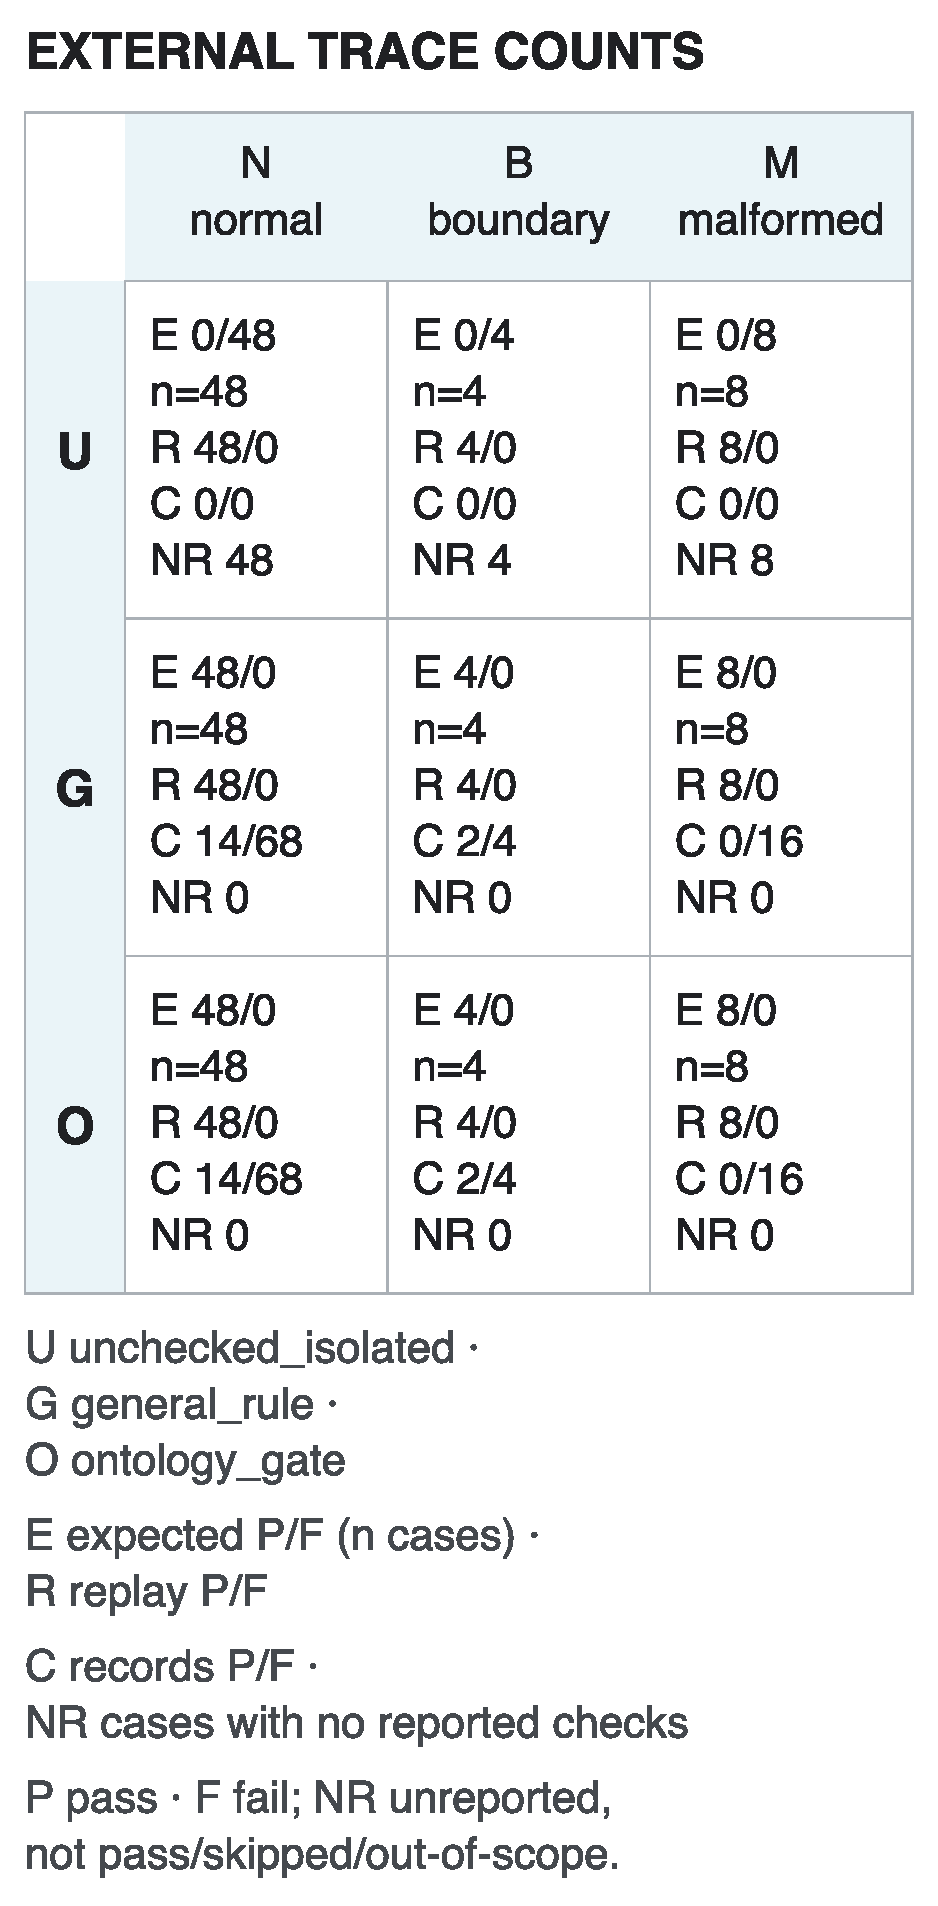
\includegraphics[width=\columnwidth]{../../figures/fig_disclosure_signals.pdf}
\caption{조건 및 계층별 NPC-DISC-1 분포(E/R: 기대 일치 및 리플레이, C: 정책 PASS/FAIL, NR: 미보고 검사).}
\Description{실험 조건 및 계층별 NPC-DISC-1 기대 일치·리플레이·정책 통과·미보고 분포 그림.}
\label{fig:disclosure-signals}
\end{figure}

\subsection{확장 0-LLM 공학 감사 (A1--A4, B)}
표~\ref{tab:extended-full}은 다중 오류 수렴, 스케일링, 추적성, Godot~4.7.1 장기 실행 안정성(그림~\ref{fig:engine-cutscenes}), 우회 필터 감사를 요약한다.

\begin{table*}[!tbp]
\caption{독립 분모 0-LLM 공학 감사 요약 (A1--A4, B)}
\label{tab:extended-full}
\centering
\footnotesize
\begin{tabularx}{\textwidth}{@{}>{\raggedright\arraybackslash}p{0.20\textwidth}>{\raggedright\arraybackslash}p{0.21\textwidth}>{\raggedright\arraybackslash}X@{}}
\toprule
\textbf{감사 항목} & \textbf{독립 분모 / 범위} & \textbf{검증된 결정론적 결과 (0 LLM 호출)} \\
\midrule
\textbf{A1} 다중 오류 수렴 & 예산당 352건 ($K{\in}\{0..3\}$, 1,408실행) + 128가드 & 안전 커밋: $K{=}0$ 0/352, $K{\ge}1$ 124/352 (35.23\%, 위험 0/1,408); \texttt{repairable\_multi} 96/96 ($K{=}1$); \texttt{conflict\_pair} 교차 시도 0/96 (주기-2 진동 96/96) vs.\ 동일 패스 가드 128/128 동결. \\
\textbf{A2} 지연 스케일링 & $N{\in}[10,2000]$ 사실 ($N{>}500$서 차수$\le$100), $R{\in}[4,256]$ 방 & $N{=}2000$ 기준 검증기 p95 0.0042\,ms (유효) / 0.0751\,ms (다중오류); $\rho$ p95 0.0317--0.0389\,ms; $R{=}256$ 폐쇄/BFS p95 0.312--0.478\,ms; SHA-256 검증 7.01\,ms; JSONL 리플레이 881.0\,ms. \\
\textbf{A3} 추적성 결함 & 시드 결함 4,656건(+N/A 1,584), 불변 3,744, \texttt{TR05} & 시드 결함 민감도 4,656/4,656 (100.00\%); 불변 오경보 0/3,744 (0.00\%); \texttt{TR05} 정방향 12/12, 역방향 10/10 직접 파일; 인간 Krippendorff $\alpha$ 미측정 (평가자 0명). \\
\textbf{A4} Godot~4.7.1 장기 실행 & 거부 코드 11건 + 1,600틱 (200에피소드) & 거부 코드 9/9 (100\%) 실행; 상태 격리 11/11; 트레이스 일관성 1,600/1,600; \texttt{step\_commit} p95 0.708\,ms; 정적 메모리 증감 $-268$\,B; 누수 0건. \\
\textbf{B} 우회 필터 (영/한) & 88건 (영 44, 한 44; \texttt{keeper\_secret}) & 재현율 / 양성 오거부율(FRR) / p95: ID전용 0.0\% / 0.0\% / 0.032\,ms; 별칭 61.1\% (22/36) / 11.1\% (4/36) / 0.041\,ms; LOO TF-IDF 97.2\% (35/36) / \textbf{58.3\% (21/36)} / 0.705\,ms. \\
\bottomrule
\end{tabularx}
\end{table*}

\begin{figure*}[!tbp]
\centering
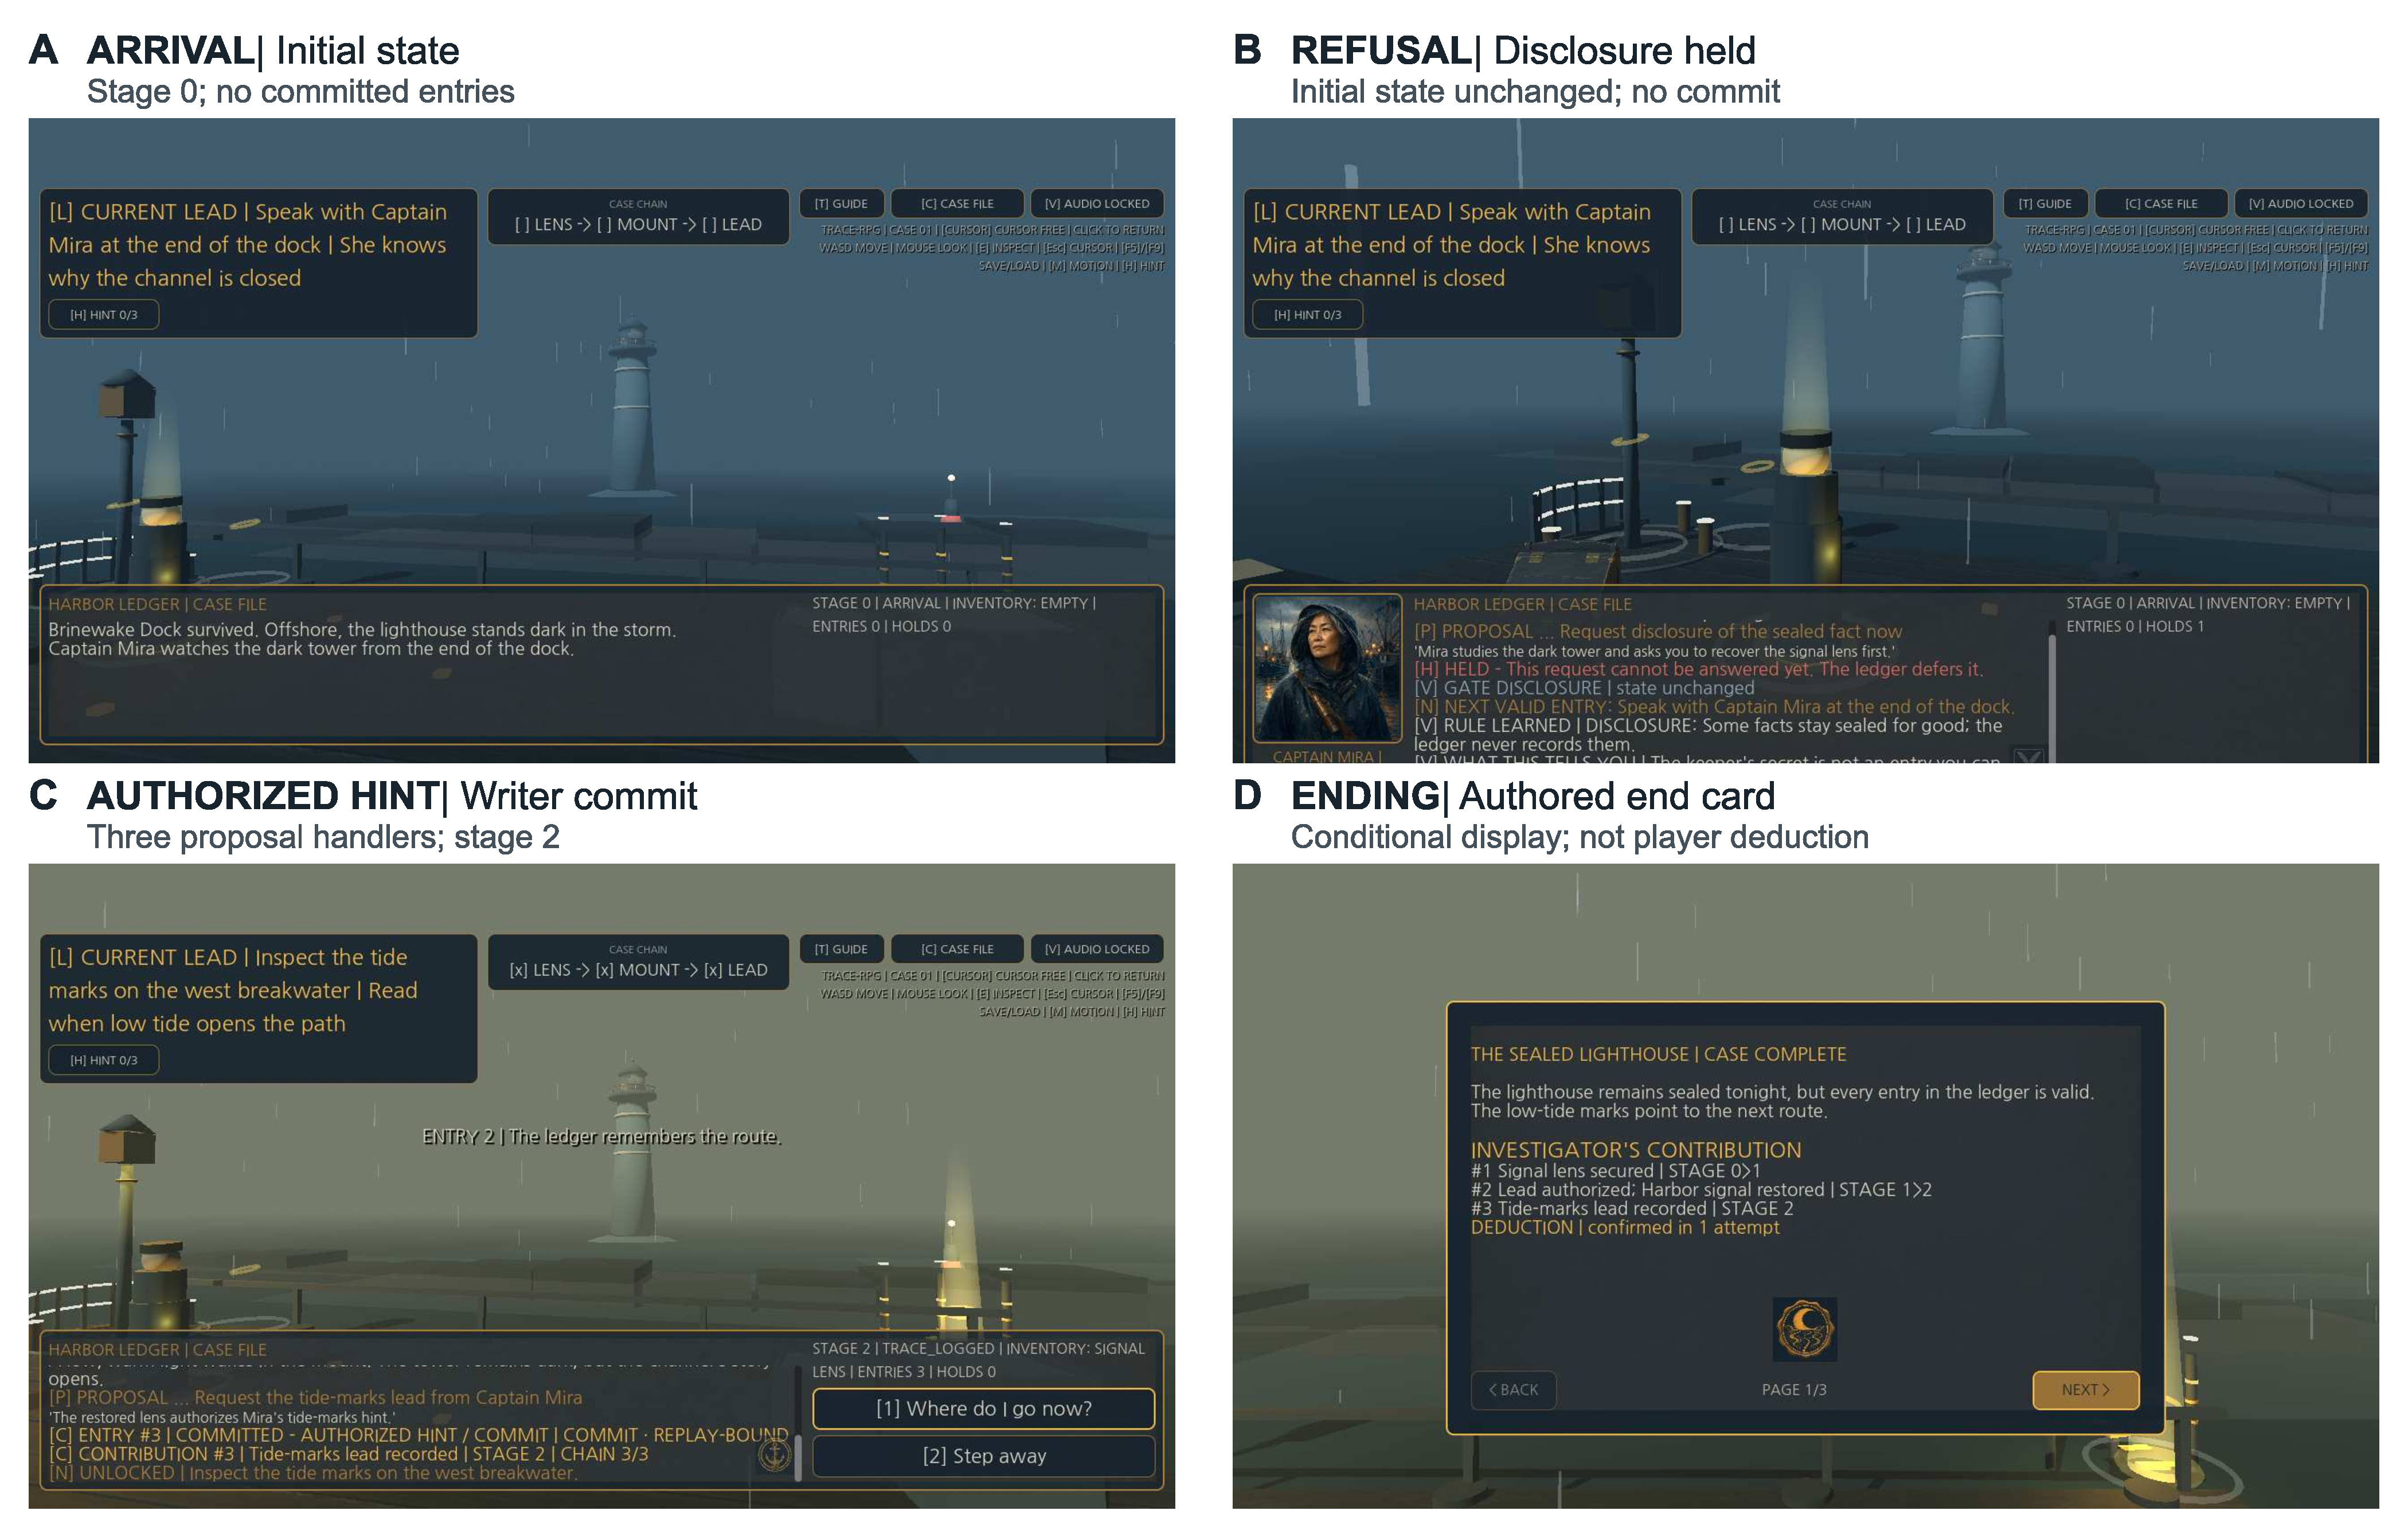
\includegraphics[width=0.90\textwidth]{../../figures/fig_engine_cutscenes.pdf}
\caption{네이티브 Godot~4.7.1 공학 캡처: (A) 초기 도착, (B) 상태 불변 비밀 공개 거부, (C) 2단계 인가 힌트, (D) 조건부 종료 카드. 사용자 효능이 아닌 렌더 상태 일치를 검증한다.}
\Description{네이티브 Godot 4.7.1 4분할 스크린샷: 초기 도착, 비밀 공개 거부, 2단계 힌트, 조건부 종료 화면.}
\label{fig:engine-cutscenes}
\end{figure*}

\subsection{제한된 확률적 제안기 파일럿}
\textbf{v5 2단계 수집}(배정 20건: $5{\times}2{\times}2$, $K{=}0$)에서는 20/20건 수신, 10/20건 파싱 통과(Luna 9/10, Terra 1/10), 8/20건 게이트 통과(표~\ref{tab:v5-summary}, 그림~\ref{fig:paired-feedback-flow}), 7/20건 목표 도달을 기록했다. \textbf{네이티브 단일 퀘스트 파일럿}(배정 8건)에서는 5/8건 목표 도달, 위험 커밋 0/16, 의미 리플레이 7/7 유효, 신규 Godot 재실행 6/6 유효를 기록했다(행 1 controller-v3 오류 1건, 온톨로지 타임아웃 2건).

\begin{table}[!tbp]
\caption{v5 합성 수집 결과 (셀당 배정 5건; 파싱 실패 포함)}
\label{tab:v5-summary}
\centering
\footnotesize
\begin{tabularx}{\columnwidth}{@{}ll*{4}{>{\centering\arraybackslash}X}@{}}
\toprule
\textbf{셀렉터} & \textbf{신호} & \textbf{수신} & \textbf{게이트} & \textbf{목표} & \textbf{파싱실패} \\
\midrule
\texttt{gpt-5.6-luna} & Detailed & 5/5 & 4/5 & 3/5 & 1/5 \\
\texttt{gpt-5.6-luna} & Generic  & 5/5 & 3/5 & 3/5 & 0/5 \\
\texttt{gpt-5.6-terra} & Detailed & 5/5 & 0/5 & 0/5 & 5/5 \\
\texttt{gpt-5.6-terra} & Generic  & 5/5 & 1/5 & 1/5 & 4/5 \\
\bottomrule
\end{tabularx}
\end{table}

\begin{figure}[!tbp]
\centering
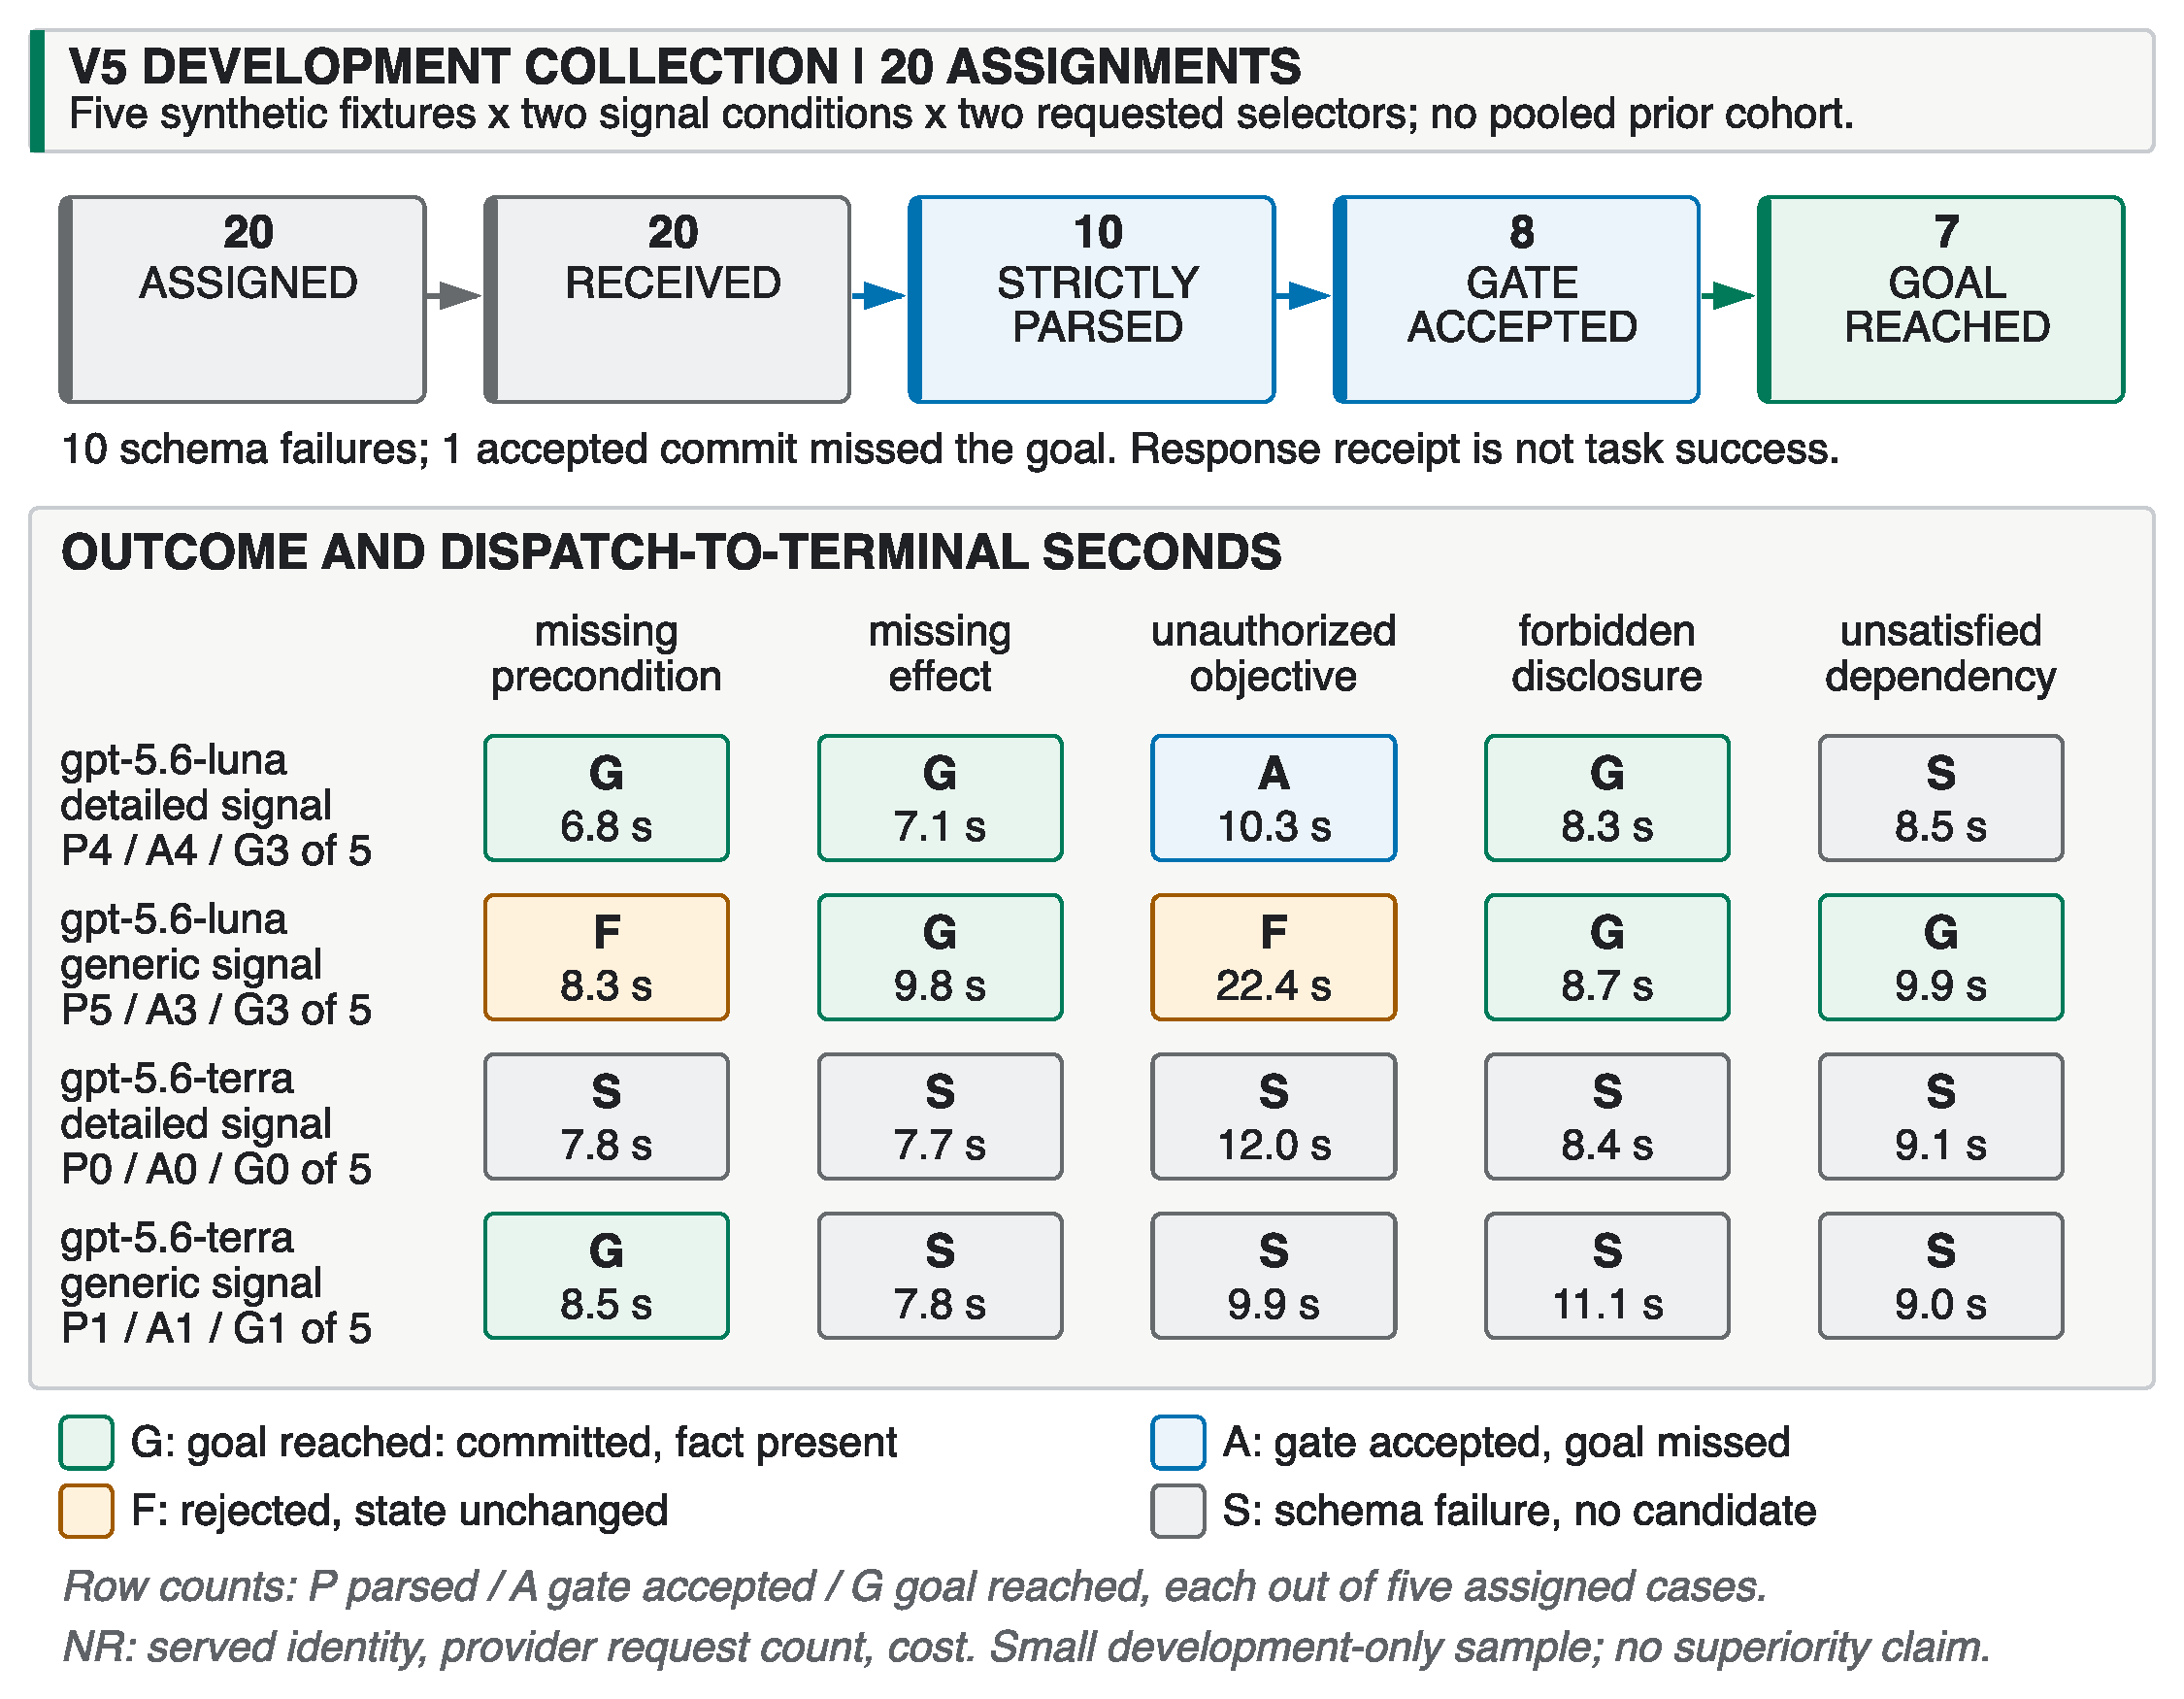
\includegraphics[width=\columnwidth]{../../figures/fig_paired_feedback_flow.pdf}
\caption{v5 배정 20건 전체 결과 흐름: 스키마 실패 10건을 분모에 보존하며, 게이트 통과 8건 중 7건이 목표에 도달했다.}
\Description{v5 배정 20건 결과 흐름도: 스키마 실패 10건, 게이트 통과 8건, 목표 달성 7건.}
\label{fig:paired-feedback-flow}
\end{figure}

\subsection{다중 홉 온톨로지 폐쇄 (3개 월드 48건)}\label{sec:multihop-eval}
단일 홉 정보 공개 60건 검사가 \texttt{general\_rule}과 \texttt{ontology\_gate}의 무회귀 동률(60/60)을 확인한 반면, 다단계 역할 상속과 사실 파생 연쇄는 추론적 폐쇄를 요구한다. 세 결정론적 퀘스트 월드(\texttt{sealed-}\allowbreak\texttt{lighthouse-}\allowbreak\texttt{v1}, \texttt{sunken-}\allowbreak\texttt{archive-}\allowbreak\texttt{v1}, \texttt{clockwork-}\allowbreak\texttt{observatory-}\allowbreak\texttt{v1})에 걸쳐 1홉(16건), 사실 파생(16건), 역할 상속(16건) 총 48건(위험 37, 허용 11)을 구성한 결과(표~\ref{tab:multihop-ontology}), \texttt{flat\_}\allowbreak\texttt{1hop\_}\allowbreak\texttt{rule}은 정확도 41.7\%(9 TP, 11 TN, 위험 누출 FN 28, FP 0)에 그쳤으나 \texttt{ontology\_}\allowbreak\texttt{multihop\_}\allowbreak\texttt{gate}는 100.0\%(37 TP, 11 TN, FN 0, FP 0)를 달성해 누출 28건을 제거하고 3개 월드 모두 \textbf{I1--I4}를 통과했다.

\begin{table}[!tbp]
\caption{다중 홉 인식론·공개 폐쇄 벤치마크 (3개 퀘스트 월드 48건)}
\label{tab:multihop-ontology}
\centering
\footnotesize
\setlength{\tabcolsep}{3.5pt}
\begin{tabularx}{\columnwidth}{@{}>{\raggedright\arraybackslash}X*{5}{c}@{}}
\toprule
\textbf{게이트 변형} & \textbf{정확도} & \textbf{TP} & \textbf{TN} & \textbf{FN(누출)} & \textbf{FP} \\
\midrule
\texttt{flat\_}\allowbreak\texttt{1hop\_}\allowbreak\texttt{rule} & 41.7\% & 9 & 11 & 28 & 0 \\
\texttt{ontology\_}\allowbreak\texttt{multihop\_}\allowbreak\texttt{gate} & \textbf{100.0\%} & \textbf{37} & 11 & \textbf{0} & 0 \\
\bottomrule
\end{tabularx}
\end{table}

\subsection{라이브 다중 퀘스트 제안기 평가 (2개 Gemini 모델, 24에피소드)}\label{sec:multiquest-live}
{\sloppy 격리된 빈 디렉터리 Antigravity CLI 샌드박스(\texttt{cli\_}\allowbreak\texttt{version~1.5.11}, 엄격 \texttt{--json-}\allowbreak\texttt{schema}, $K{\in}\{0..2\}$, 제공자 리비전 및 시드 미인증 명시)에서 2종 라이브 모델(\texttt{gemini-3.8-}\allowbreak\texttt{flash-}\allowbreak\texttt{medium}, \texttt{gemini-4-}\allowbreak\texttt{hydrogen-}\allowbreak\texttt{medium}), 2종 게이트 표현(\texttt{general\_}\allowbreak\texttt{rule}, \texttt{ontology\_}\allowbreak\texttt{gate}), 3개 퀘스트, 2회 반복을 교차해 24에피소드(129턴, 4,606,387토큰, 5,065.47초)를 실행했다. 표~\ref{tab:multiquest-live}는 모델·조건·퀘스트별 결과를 보인다. 두 모델 모두 \textbf{0}건의 위험 커밋을 유지한 채 스키마 통과 후 위험 턴 70건을 차단했고(Flash 21, Hydrogen 49), 24/24건 엄격 의미 리플레이(\texttt{allow\_}\allowbreak\texttt{defaults=}\allowbreak\texttt{false})를 통과했다. 검증기 거부 71건 중 69건이 \texttt{NPC\_}\allowbreak\texttt{KNOWLEDGE\_}\allowbreak\texttt{VIOLATION}(외 \texttt{UNSATISFIED\_}\allowbreak\texttt{PRECONDITION} 1, \texttt{QUEST\_}\allowbreak\texttt{STAGE\_}\allowbreak\texttt{VIOLATION} 1)였기 때문에 정리~2에 따라 \texttt{repaired\_}\allowbreak\texttt{steps}는 0으로 유지되어 라이브 제안기의 상태 세탁을 원천 차단했다. Flash는 7/12 목표 달성 및 파싱 실패 0건을, Hydrogen은 0/12 목표 및 150초 타임아웃 2건(분모 보존)을 기록했다.\par}

\begin{table*}[!tbp]
\caption{라이브 다중 퀘스트 Antigravity CLI 평가 (24에피소드, 129턴, 엄격 \texttt{--json-schema}; 리비전·시드 미인증)}
\label{tab:multiquest-live}
\centering
\footnotesize
\setlength{\tabcolsep}{4pt}
\begin{tabularx}{\textwidth}{@{}>{\raggedright\arraybackslash}X*{6}{c}r@{}}
\toprule
\textbf{구분 (에피소드 / 턴)} & \textbf{목표} & \textbf{커밋} & \textbf{파싱실패} & \textbf{위험차단} & \textbf{위험커밋} & \textbf{리플레이} & \textbf{토큰 / 지연} \\
\midrule
\texttt{gemini-3.8-}\allowbreak\texttt{flash-}\allowbreak\texttt{medium} (\texttt{general\_rule}, 6 / 26) & 4/6 & 18/26 & 0 & 8 & \textbf{0} & 6/6 & 993,141 / 1,000.9초 \\
\texttt{gemini-3.8-}\allowbreak\texttt{flash-}\allowbreak\texttt{medium} (\texttt{ontology\_gate}, 6 / 31) & 3/6 & 18/31 & 0 & 13 & \textbf{0} & 6/6 & 998,064 / 1,306.5초 \\
\texttt{gemini-4-}\allowbreak\texttt{hydrogen-}\allowbreak\texttt{medium} (\texttt{general\_rule}, 6 / 36) & 0/6 & 10/36 & 2 & 24 & \textbf{0} & 6/6 & 1,223,288 / 1,339.7초 \\
\texttt{gemini-4-}\allowbreak\texttt{hydrogen-}\allowbreak\texttt{medium} (\texttt{ontology\_gate}, 6 / 36) & 0/6 & 11/36 & 0 & 25 & \textbf{0} & 6/6 & 1,391,894 / 1,418.4초 \\
\midrule
퀘스트: \texttt{sealed-lighthouse-v1} (8 / 39) & 3/8 & 13/39 & 2 & 24 & \textbf{0} & 8/8 & 1,302,715 / 1,509.6초 \\
퀘스트: \texttt{sunken-archive-v1} (8 / 48) & 0/8 & 17/48 & 0 & 31 & \textbf{0} & 8/8 & 1,821,567 / 1,962.5초 \\
퀘스트: \texttt{clockwork-observatory-v1} (8 / 42) & 4/8 & 27/42 & 0 & 15 & \textbf{0} & 8/8 & 1,482,105 / 1,593.4초 \\
\midrule
\textbf{전체 합계 (24 / 129)} & \textbf{7/24} & \textbf{57/129} & \textbf{2} & \textbf{70} & \textbf{0} & \textbf{24/24} & \textbf{4,606,387 / 5,065.5초} \\
\bottomrule
\end{tabularx}
\end{table*}

\subsection{2차 의미 우회 검증기와 인간 평가·Croissant 패키징}\label{sec:auditb-human}
Audit~\textbf{B} 88건 전체(명시 16, 우회 36, 정상 36; 한·영 각 44건)에서 LOO TF-IDF의 58.3\% 양성 오거부율(FRR)을 해소하기 위해(표~\ref{tab:auditb-verifiers}), 보정 \texttt{rule\_hybrid}는 FRR 2.8\%($F_1{=}0.809$)로 개선되었고, 라이브 2차 \texttt{gemini-3.8-}\allowbreak\texttt{flash-}\allowbreak\texttt{medium}은 \textbf{0.0\% FRR(0/36)}에서 우회 35/36건(97.2\%, $F_1{=}0.990$, 오류 0건)을 탐지했다(비과학적 탐색용 로컬 0.8B 자문 기준선은 우회 0/36). 아울러 \texttt{TR01--TR06} 인간 추적성 평가는 실제 \texttt{execute\_bounded\_step} 트레이스와 해시가 결속된 36항목 블라인드 패킷(\texttt{AWAITING\_}\allowbreak\texttt{HUMAN\_}\allowbreak\texttt{RATERS}, $N{=}0$, 합성 라벨 0건) 및 Croissant~1.0(6/6 SHA-256 일치)으로 패키징하였다.

\begin{table*}[!tbp]
\caption{Audit~B 88건 한·영 2차 의미 우회 검증기 비교 (기존 결정론 기준선 대 보정·라이브 2차 검증기)}
\label{tab:auditb-verifiers}
\centering
\footnotesize
\setlength{\tabcolsep}{4pt}
\begin{tabularx}{\textwidth}{@{}>{\raggedright\arraybackslash}X*{6}{c}@{}}
\toprule
\textbf{검증기 계층} & \textbf{명시 (16)} & \textbf{우회 (36)} & \textbf{양성 FRR (36)} & \textbf{정밀도} & \textbf{재현율} & \textbf{$F_1$ / 상태} \\
\midrule
LOO TF-IDF (기존 결정론) & 16/16 (100\%) & 35/36 (97.2\%) & 21/36 (58.3\%) & 0.708 & 0.981 & 0.823 / 결정론 \\
\texttt{rule\_hybrid} (보정 결정론) & 16/16 (100\%) & 20/36 (55.6\%) & 1/36 (2.8\%) & 0.973 & 0.692 & 0.809 / 결정론 \\
로컬 0.8B Jev (미보정 자문용) & 16/16 (100\%) & 0/36 (0.0\%) & 0/36 (0.0\%) & 1.000 & 0.308 & 0.471 / 자문용 \\
\texttt{gemini-4-}\allowbreak\texttt{hydrogen-}\allowbreak\texttt{medium} (라이브) & 16/16 (100\%) & 29/36 (80.6\%) & \textbf{0/36 (0.0\%)} & \textbf{1.000} & 0.865 & 0.928 / 9 오류 \\
\texttt{gemini-3.8-}\allowbreak\texttt{flash-}\allowbreak\texttt{medium} (라이브) & 16/16 (100\%) & \textbf{35/36 (97.2\%)} & \textbf{0/36 (0.0\%)} & \textbf{1.000} & \textbf{0.981} & \textbf{0.990 / 0 오류} \\
\bottomrule
\end{tabularx}
\end{table*}
